\section{Esempi quiz secondo parziale}

\begin{figure}[!ht]
\centering
	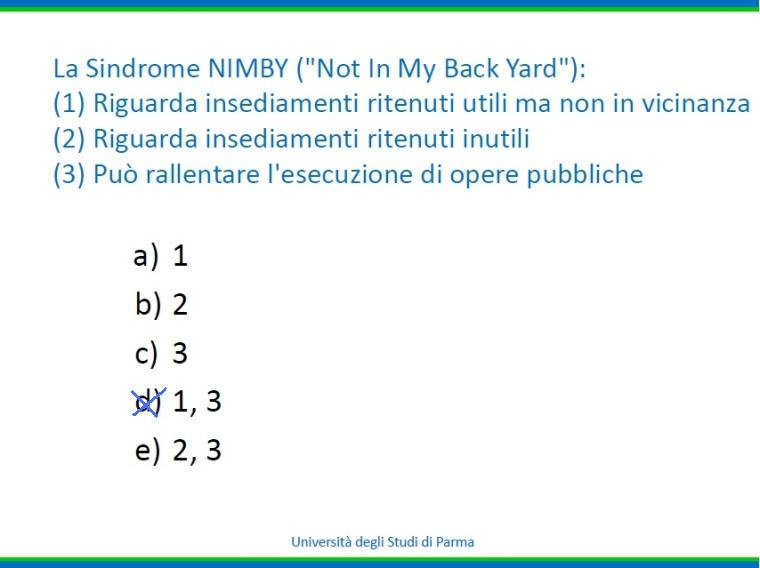
\includegraphics[width=0.5\textwidth]{25/image1.jpeg}
	\end{figure}

La Sindrome NIMBY si riferisce a delle opere ritenute utili ma, con un
approccio egoistico, non volute nelle vicinanze di residenza delle
persone interessate. (Risposta corretta: D)
\\\\
\begin{figure}[!ht]
\centering
	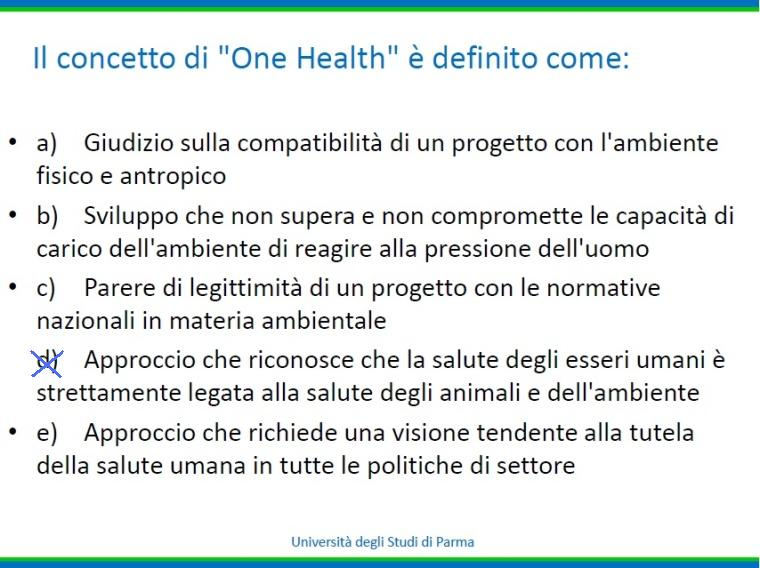
\includegraphics[width=0.5\textwidth]{25/image2.jpeg}
	\end{figure}

(Risposta corretta: D)

\begin{figure}[!ht]
\centering
	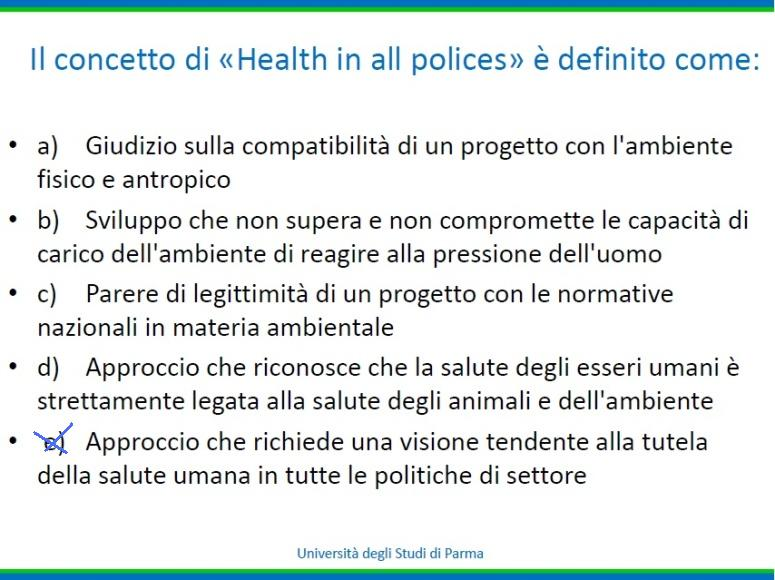
\includegraphics[width=0.5\textwidth]{25/image3.jpeg}
	\end{figure}

Per quanto quello di \textless{}\textless{}Health in all
polices\textgreater{}\textgreater{} sia un concetto assolutamente logico
e che risuona nella teoria, nella pratica delle politiche non sanitarie
(ambientali, sociali, economiche) è in realtà di difficile applicazione,
in quanto entrano in gioco altri interessi che sono in conflitto con
l'interesse della tutela della salute. (Risposta corretta: E)
\\\\
\begin{figure}[!ht]
\centering
	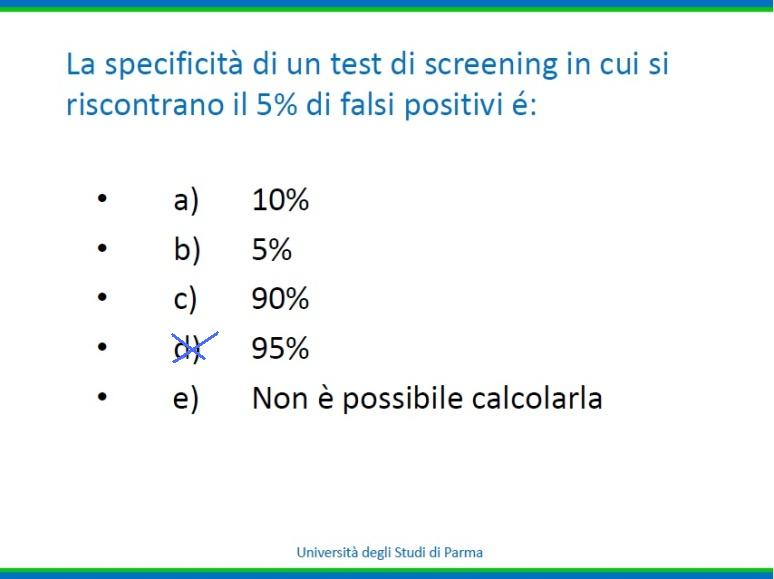
\includegraphics[width=0.5\textwidth]{25/image4.jpeg}
	\end{figure}

La sezione dedicata allo screening è un argomento d'esame ricorrente sia
nei quiz che nell'esame orale, in quanto argomento cardine della sanità
pubblica, della prevenzione e dell'epidemiologia. è importante conoscere
le definizioni e saper calcolare specificità, sensibilità, valore
predittivo positivo e valore predittivo negativo. (Risposta corretta: D)

Un'altra domanda ricorrente riguarda quale dei due gruppi (sensibilità e
specificità o valori predittivi positivo e negativo) è influenzato dalla
prevalenza di una malattia. Ad essere influenzati dalla prevalenza sono
i valori predittivi (che cambiano valore a seconda di quanto sia
prevalente la malattia) mentre specificità e sensibilità non lo sono.
\\\\
\begin{figure}[!ht]
\centering
	
\includegraphics[width=0.5\textwidth]{25/image5.jpeg}
	\end{figure}

(Risposta corretta: A)
\\\\
\begin{figure}[!ht]
\centering
	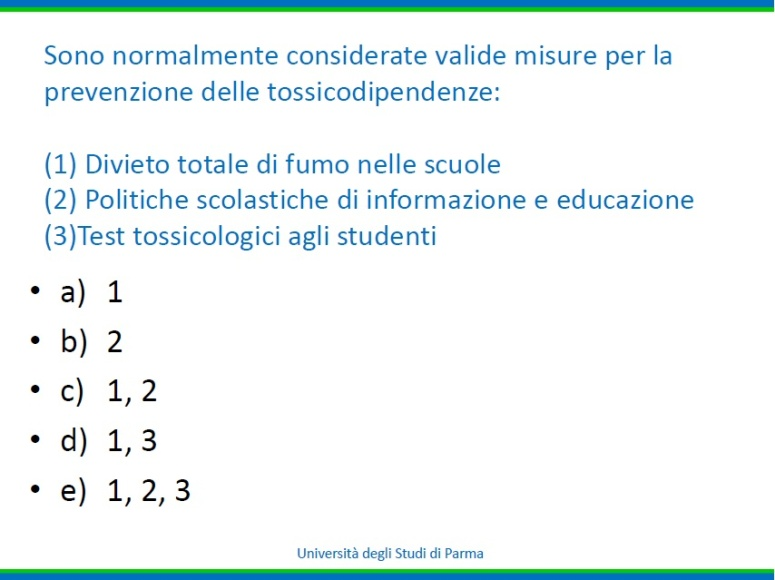
\includegraphics[width=0.5\textwidth]{25/image6.jpeg}
	\end{figure}

(Risposta corretta: C)
\\\\
\begin{figure}[!ht]
\centering
	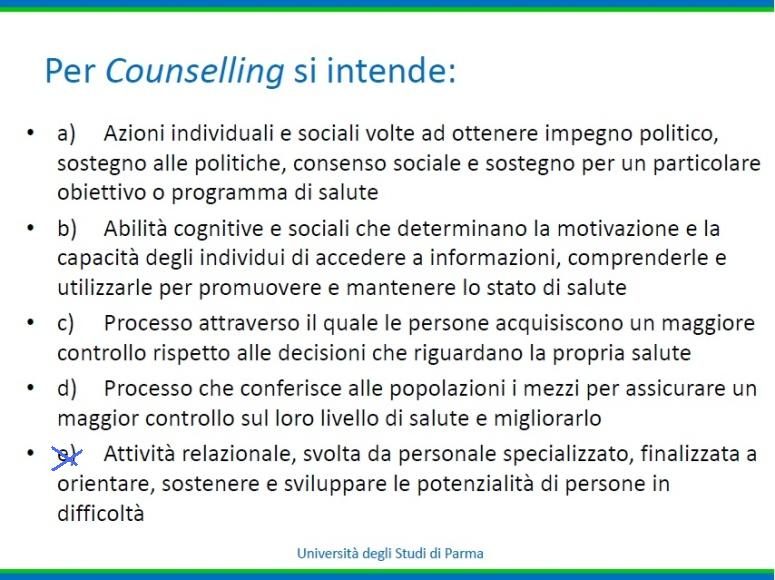
\includegraphics[width=0.5\textwidth]{25/image7.jpeg}
	\end{figure}

(Risposta corretta: E) La risposta A è la definizione di Advocacy.
\\\\
\begin{figure}[!ht]
\centering
	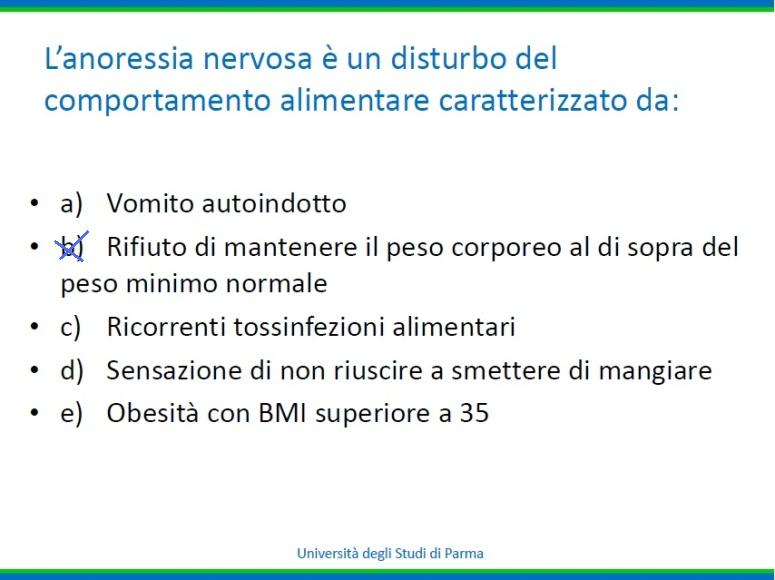
\includegraphics[width=0.5\textwidth]{25/image8.jpeg}
	\end{figure}

(Risposta corretta: B)
\\\\
\begin{figure}[!ht]
\centering
	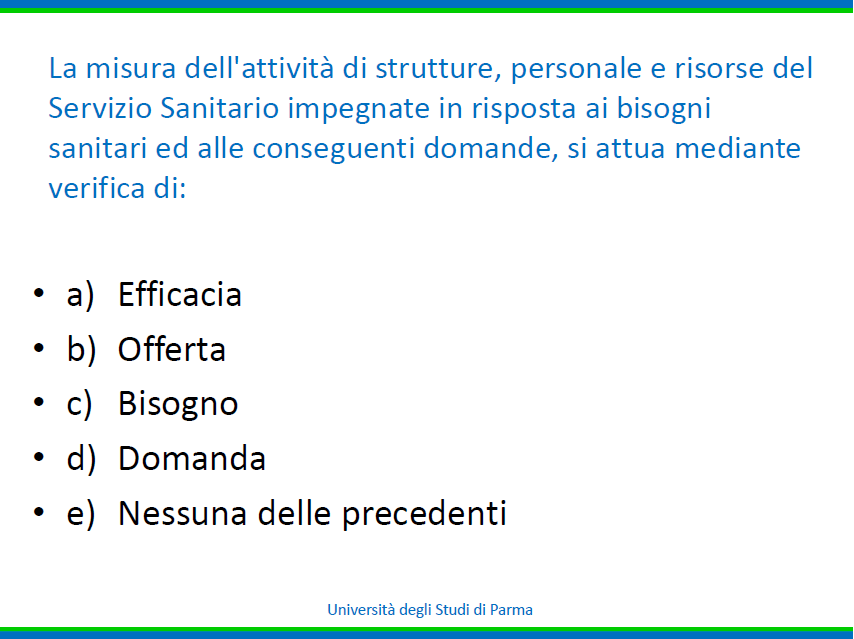
\includegraphics[width=0.5\textwidth]{25/image9.png}
	\end{figure}

(Risposta corretta: A)
\\\\
\begin{figure}[!ht]
\centering
	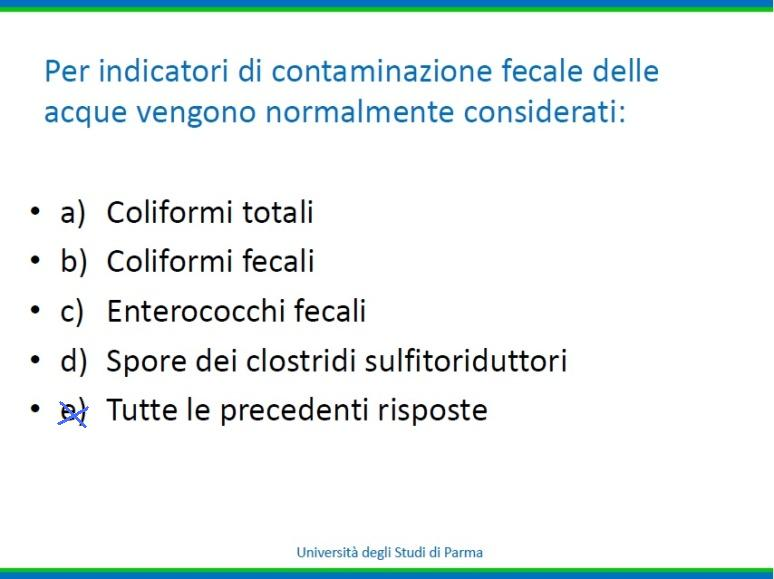
\includegraphics[width=0.5\textwidth]{25/image10.jpeg}
	\end{figure}

(Risposta corretta: E)
\\\\
\begin{figure}[!ht]
\centering
	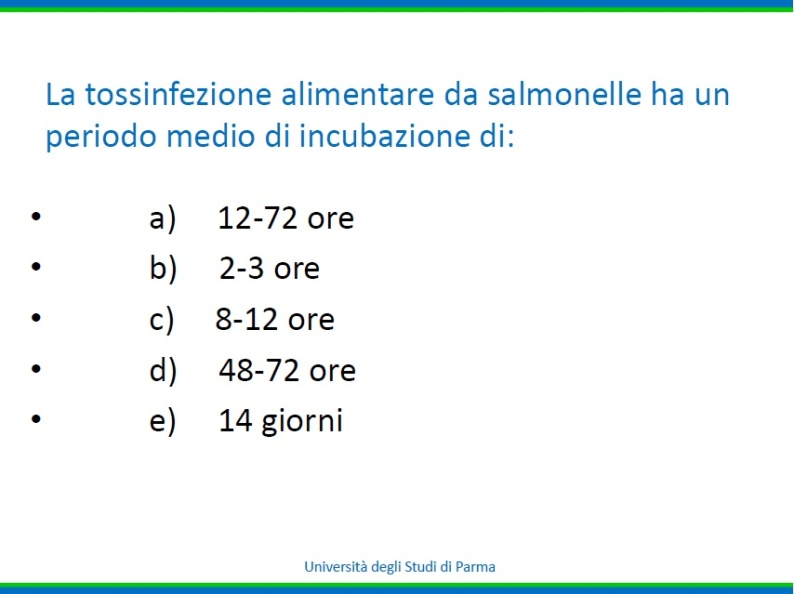
\includegraphics[width=0.5\textwidth]{25/image11.jpeg}
	\end{figure}

Fare attenzione alla differenza tra infezione alimentare e tossinfezione
alimentare in quanto cambiano i microorganismi, i tempi di incubazione e
di conseguenza le misure di profilassi e di prevenzione. (Risposta
corretta: A)
